\let\negmedspace\undefined
\let\negthickspace\undefined
\documentclass[journal,12pt,twocolumn]{IEEEtran}
\usepackage{cite}
\usepackage{amsmath,amssymb,amsfonts,amsthm}
\usepackage{algorithmic}
\usepackage{graphicx}
\usepackage{textcomp}
\usepackage{xcolor}
\usepackage{txfonts}
\usepackage{listings}
\usepackage{enumitem}
\usepackage{mathtools}
\usepackage{gensymb}
\usepackage{comment}
\usepackage[breaklinks=true]{hyperref}
\usepackage{tkz-euclide} 
\usepackage{listings}
\usepackage{gvv}                                        
\def\inputGnumericTable{}                                 
\usepackage[latin1]{inputenc}                                
\usepackage{color}                                            
\usepackage{array}                                            
\usepackage{longtable}                                       
\usepackage{calc}                                             
\usepackage{multirow}                                         
\usepackage{hhline}                                           
\usepackage{ifthen}                                           
\usepackage{lscape}

\newtheorem{theorem}{Theorem}[section]
\newtheorem{problem}{Problem}
\newtheorem{proposition}{Proposition}[section]
\newtheorem{lemma}{Lemma}[section]
\newtheorem{corollary}[theorem]{Corollary}
\newtheorem{example}{Example}[section]
\newtheorem{definition}[problem]{Definition}
\newcommand{\BEQA}{\begin{eqnarray}}
\newcommand{\EEQA}{\end{eqnarray}}
\newcommand{\define}{\stackrel{\triangle}{=}}
\theoremstyle{remark}
\newtheorem{rem}{Remark}
\begin{document}

\bibliographystyle{IEEEtran}
\vspace{3cm}

\title{GATE-2023, EC-35}
\author{EE23BTECH11033- JASWANTH KILLANA}
\maketitle
\newpage
\bigskip

\renewcommand{\thefigure}{\theenumi}
\renewcommand{\thetable}{\theenumi}
\textbf{Question}:\\
In the circuit shown below, switch S was closed for a long time. If the switch is opened at t=0, the maximum magnitude of the voltage $V_R$ in volts is. (round off to nearest integer).\\
\begin{figure}[th]
\centering
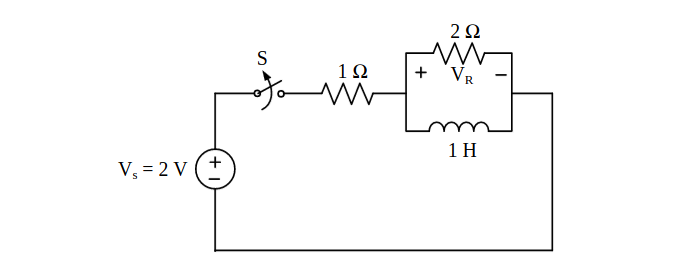
\includegraphics[width=\linewidth]{gate.png}
\caption{}
\label{}
\end{figure}
\textbf{solution} :
here\begin{table}[!ht]
 \centering
  \begin{tabular}{|c|c|c|}
\hline
\textbf{parameter}& \textbf{description}& \textbf{value}
\\\hline
\multirow{3}{1em}\\$l$&length&$50m$
\\\hline
$b$&breadth&$0.25m$
\\\hline
$h$&height&$0.5m$
\\\hline
$y(n)$& sum of volume&$6.25m^3$ 
\\\hline
\end{tabular}


   \caption{input parameters}
   \label{GATE-2023,EC-35}
   \end{table}
at $t<0$, switch is closed\\
after $t=0$, switch is opened\\
for an inductor \begin{align}
i\brak{0^{+}}=i\brak{0^{-}}
\end{align}
apply KVL before $t<0$\\
inductor acts as wire\\
-\begin{align}
-2V+i\brak{0^-}&=0\\
\implies i\brak{0^-}=i\brak{0^+}&=2A
\end{align}
after $t=0$;\\
KVL in loop of inductor and  $2$\ohm \quad resistor\\
\\ let i be current in the loop in anti clockwise direction\\
\begin{align}
L\frac{di}{dt}&=-2i\\
\implies\frac{di}{i}&=\frac{-2dt}{L}\\
\int_{i\brak{0^+}}^{i\brak{t}}{\frac{1}{i}\,di}&=\int_{0}^{t}{\frac{-2}{L}\,dt}\\
ln\brak{\frac{i\brak{t}}{2}}&=-2t\\
\implies i\brak{t}&=2\cdot{e^{-2t}}\\
V_{R}&=2i\brak{t}V\\
 &=4\cdot{e^{-2t}}V
 \end{align}
 \begin{align}
 As, t\xrightarrow{}\infty\\
 e^{-2t}\xrightarrow{}1\\
 \abs{V_R\brak{max}}=4V
\end{align}
\end{document}

